\documentclass[
	ngerman,
	toc=listof, % Abbildungsverzeichnis sowie Tabellenverzeichnis in das Inhaltsverzeichnis aufnehmen
	toc=bibliography, % Literaturverzeichnis in das Inhaltsverzeichnis aufnehmen
	footnotes=multiple, % Trennen von direkt aufeinander folgenden Fußnoten
	parskip=half, % vertikalen Abstand zwischen Absätzen verwenden anstatt horizontale Einrückung von Folgeabsätzen
	numbers=noendperiod % Den letzten Punkt nach einer Nummerierung entfernen (nach DIN 5008)
]{scrartcl}
\pdfminorversion=5 % erlaubt das Einfügen von pdf-Dateien bis Version 1.7, ohne eine Fehlermeldung zu werfen (keine Garantie für fehlerfreies Einbetten!)

% Dokumenteninformationen ----------------------------------------------------
\newcommand{\titel}{Anforderungsanalyse}
\newcommand{\untertitel}{Studienarbeit \semester}
\newcommand{\kompletterTitel}{\titel{} \\ \untertitel}
\newcommand{\datum}{\today}

\newcommand{\vorlagenOrdner}{../../99_Vorlagen} % Falls im Unterordner ../ vorne hinzufügen

\newcommand{\betriebLogo}{\vorlagenOrdner/Bilder/logo}

% Konfiguration -------------------------------------------------------------
\newcommand{\autoren}{
    \author{
        Schmid, Mike\\
        \texttt{sgschwin@hsr.ch}
        \and
        Schlatter, Janik\\
        \texttt{jschlatt@hsr.ch}
    }
}

\newcommand{\betreuer}{
    Stettler Beat\\
    \scriptsize \texttt{\url{beat.stettler@hsr.ch}}
    \normalsize
}

\newcommand{\schmid}{
    Mike Schmid\\
    \url{mschmid@hsr.ch}
    \normalsize
}

\newcommand{\schlatter}{
    Janik Schlatter\\
    \scriptsize \url{jschlatt@hsr.ch}
    \normalsize
}

\newcommand{\autorenNamen}{
    M. Schmid, J. Schlatter
}

\newcommand{\semester}{FS-2020}
\newcommand{\betriebName}{\textsc{HSR} Hochschule für Technik Rapperswil} % Metadaten zu diesem Dokument (Autor usw.)
% !TEX root = ../Projektdokumentation.tex

% Anpassung an Landessprache ---------------------------------------------------
\usepackage[english, main=ngerman]{babel} % \selectlanguage{english} if  needed

% Umlaute ----------------------------------------------------------------------
%   Umlaute/Sonderzeichen wie äüöß direkt im Quelltext verwenden (CodePage).
%   Erlaubt automatische Trennung von Worten mit Umlauten.
% ------------------------------------------------------------------------------
\usepackage[T1]{fontenc}
\usepackage[utf8]{inputenc}
\usepackage{textcomp} % Euro-Zeichen etc.

% Schrift ----------------------------------------------------------------------
\usepackage{lmodern} % bessere Fonts
\usepackage{relsize} % Schriftgröße relativ festlegen

% Tabellen ---------------------------------------------------------------------
\PassOptionsToPackage{table}{xcolor}
\usepackage{tabularx}
\usepackage{tabulary}
\usepackage{booktabs}
\usepackage{makecell}
\usepackage[table,xcdraw]{xcolor}
% für lange Tabellen
\usepackage{longtable}
\usepackage{array}
\usepackage{ragged2e}
\usepackage{lscape}
% Multi Columns
\usepackage{multicol}

% Grafiken ---------------------------------------------------------------------
\usepackage[dvips,final]{graphicx} % Einbinden von JPG-Grafiken ermöglichen
\usepackage{graphics} % keepaspectratio
\usepackage{floatflt} % zum Umfließen von Bildern
\graphicspath{{Bilder/}} % hier liegen die Bilder des Dokuments

% Sonstiges --------------------------------------------------------------------
\usepackage[titles]{tocloft} % Inhaltsverzeichnis DIN 5008 gerecht einrücken
\usepackage{enumitem} % anpassbare Enumerates/Itemizes
\usepackage{xspace} % sorgt dafür, dass Leerzeichen hinter parameterlosen Makros nicht als Makroendezeichen interpretiert werden

\usepackage{makeidx} % für Index-Ausgabe mit \printindex
\usepackage[printonlyused]{acronym} % es werden nur benutzte Definitionen aufgelistet

% Einfache Definition der Zeilenabstände und Seitenränder etc.
\usepackage{setspace}
\usepackage{geometry}

% Symbolverzeichnis
\usepackage[intoc]{nomencl}
\let\abbrev\nomenclature
\renewcommand{\nomname}{Abkürzungsverzeichnis}
\setlength{\nomlabelwidth}{.25\hsize}
\renewcommand{\nomlabel}[1]{#1 \dotfill}
\setlength{\nomitemsep}{-\parsep}

\usepackage{varioref} % Elegantere Verweise. „auf der nächsten Seite“
\usepackage{url} % URL verlinken, lange URLs umbrechen etc.

\usepackage{chngcntr} % fortlaufendes Durchnummerieren der Fußnoten
% \usepackage[perpage]{footmisc} % Alternative: Nummerierung der Fußnoten auf jeder Seite neu

\usepackage{ifthen} % bei der Definition eigener Befehle benötigt
\usepackage{todonotes} % definiert u.a. die Befehle \todo und \listoftodos
\usepackage[square]{natbib} % wichtig für korrekte Zitierweise

% PDF-Optionen -----------------------------------------------------------------
\usepackage{pdfpages}
\pdfminorversion=5 % erlaubt das Einfügen von pdf-Dateien bis Version 1.7, ohne eine Fehlermeldung zu werfen (keine Garantie für fehlerfreies Einbetten!)
\usepackage[
    bookmarks,
    bookmarksnumbered,
    bookmarksopen=true,
    bookmarksopenlevel=1,
    colorlinks=true,
% diese Farbdefinitionen zeichnen Links im PDF farblich aus
    linkcolor=AOBlau, % einfache interne Verknüpfungen
    anchorcolor=AOBlau,% Ankertext
    citecolor=AOBlau, % Verweise auf Literaturverzeichniseinträge im Text
    filecolor=AOBlau, % Verknüpfungen, die lokale Dateien öffnen
    menucolor=AOBlau, % Acrobat-Menüpunkte
    urlcolor=AOBlau,
% diese Farbdefinitionen sollten für den Druck verwendet werden (alles schwarz)
    %linkcolor=black, % einfache interne Verknüpfungen
    %anchorcolor=black, % Ankertext
    %citecolor=black, % Verweise auf Literaturverzeichniseinträge im Text
    %filecolor=black, % Verknüpfungen, die lokale Dateien öffnen
    %menucolor=black, % Acrobat-Menüpunkte
    %urlcolor=black,
%
    %backref, % Quellen werden zurück auf ihre Zitate verlinkt
    pdftex,
    plainpages=false, % zur korrekten Erstellung der Bookmarks
    pdfpagelabels=true, % zur korrekten Erstellung der Bookmarks
    hypertexnames=false, % zur korrekten Erstellung der Bookmarks
    linktocpage % Seitenzahlen anstatt Text im Inhaltsverzeichnis verlinken
]{hyperref}
% Befehle, die Umlaute ausgeben, führen zu Fehlern, wenn sie hyperref als Optionen übergeben werden
\hypersetup{
    pdftitle={\titel -- \untertitel},
    pdfauthor={\autoren},
    pdfcreator={\autoren},
    pdfsubject={\titel -- \untertitel},
    pdfkeywords={\titel -- \untertitel},
}


% zum Einbinden von Programmcode -----------------------------------------------
\usepackage{listings}
\usepackage{xcolor}
\usepackage{beramono}
% Pseudocode
\usepackage{algorithmic}
\usepackage[linesnumbered,ruled]{algorithm2e}

\definecolor{hellgelb}{rgb}{1,1,0.9}
\definecolor{colKeys}{rgb}{0,0,1}
\definecolor{colIdentifier}{rgb}{0,0,0}
\definecolor{colComments}{rgb}{0,0.5,0}
\definecolor{colString}{rgb}{1,0,0}
\definecolor{bluekeywords}{rgb}{0,0,1}
\definecolor{greencomments}{rgb}{0,0.5,0}
\definecolor{redstrings}{rgb}{0.64,0.08,0.08}
\definecolor{xmlcomments}{rgb}{0.5,0.5,0.5}
\definecolor{types}{rgb}{0.17,0.57,0.68}
\definecolor{DarkPurple}{rgb}{0.4, 0.1, 0.4}
\definecolor{DarkCyan}{rgb}{0.0, 0.5, 0.4}
\definecolor{LightLime}{rgb}{0.3, 0.5, 0.4}
\definecolor{Blue}{rgb}{0.0, 0.0, 1.0}
\definecolor{AOBlau}{rgb}{0, 0.28, 0.56}
% Tabellenfärbung:
\definecolor{heading}{rgb}{0.64,0.78,0.86}
\definecolor{odd}{rgb}{0.9,0.9,0.9}

\lstset{
    float=hbp,
	basicstyle=\footnotesize,
    identifierstyle=\color{colIdentifier},
    keywordstyle=\color{colKeys},
    stringstyle=\color{colString},
    commentstyle=\color{colComments},
    backgroundcolor=\color{hellgelb},
    columns=flexible,
    tabsize=2,
    frame=single,
    extendedchars=true,
    showspaces=false,
    showstringspaces=false,
    numbers=left,
    numberstyle=\tiny,
    breaklines=true,
    breakautoindent=true,
	captionpos=b,
}
\lstdefinestyle{visual-studio-style}{
	language=[Sharp]C,
	columns=flexible,
	showstringspaces=false,
	basicstyle=\footnotesize\ttfamily, 
	commentstyle=\color{greencomments},
	morekeywords={partial, var, value, get, set},
	keywordstyle=\bfseries\color{bluekeywords},
	stringstyle=\color{redstrings},
	breaklines=true,
	breakatwhitespace=true,
	tabsize=4,
	numbers=left,
	numberstyle=\tiny\color{black},
	frame=lines,
	showspaces=false,
	showtabs=false,
	escapeinside={£}{£},
}
\lstdefinestyle{eclipse-style}{
	language=Java,  
	columns=flexible,
	showstringspaces=false,     
	basicstyle=\footnotesize\ttfamily, 
	keywordstyle=\bfseries\color{DarkPurple},
	commentstyle=\color{LightLime},
	stringstyle=\color{Blue}, 
	escapeinside={£}{£}, % latex scope within code      
	breaklines=true,
	breakatwhitespace=true,
	showspaces=false,
	showtabs=false,
	tabsize=4,
	morekeywords={length},
	numbers=left,
	numberstyle=\tiny\color{black},
	frame=lines,
}
\lstset{style=eclipse-style}
\lstdefinelanguage{cs}{
	sensitive=false,
	morecomment=[l]{//},
	morecomment=[s]{/*}{*/},
	morestring=[b]",
	morekeywords={
		abstract,event,new,struct,as,explicit,null,switch
		base,extern,object,this,bool,false,operator,throw,
		break,finally,out,true,byte,fixed,override,try,
		case,float,params,typeof,catch,for,private,uint,
		char,foreach,protected,ulong,checked,goto,public,unchecked,
		class,if,readonly,unsafe,const,implicit,ref,ushort,
		continue,in,return,using,decimal,int,sbyte,virtual,
		default,interface,sealed,volatile,delegate,internal,short,void,
		do,is,sizeof,while,double,lock,stackalloc,
		else,long,static,enum,namespace,string},
}
\lstdefinelanguage{natural}{
	sensitive=false,
	morecomment=[l]{/*},
	morestring=[b]",
	morestring=[b]',
	alsodigit={-,*},
	morekeywords={
		DEFINE,DATA,LOCAL,END-DEFINE,WRITE,CALLNAT,PARAMETER,USING,
		IF,NOT,END-IF,ON,*ERROR-NR,ERROR,END-ERROR,ESCAPE,ROUTINE,
		PERFORM,SUBROUTINE,END-SUBROUTINE,CONST,END-FOR,END,FOR,RESIZE,
		ARRAY,TO,BY,VALUE,RESET,COMPRESS,INTO,EQ},
}
\lstdefinelanguage{php}{
	sensitive=false,
	morecomment=[l]{/*},
	morestring=[b]",
	morestring=[b]',
	alsodigit={-,*},
	morekeywords={
		abstract,and,array,as,break,case,catch,cfunction,class,clone,const,
		continue,declare,default,do,else,elseif,enddeclare,endfor,endforeach,
		endif,endswitch,endwhile,extends,final,for,foreach,function,global,
		goto,if,implements,interface,instanceof,namespace,new,old_function,or,
		private,protected,public,static,switch,throw,try,use,var,while,xor
		die,echo,empty,exit,eval,include,include_once,isset,list,require,
		require_once,return,print,unset},
}
 % verwendete Packages
% !TEX root = ../Projektdokumentation.tex

% Seitenränder -----------------------------------------------------------------
\setlength{\topskip}{\ht\strutbox} % behebt Warnung von geometry
\geometry{
	a4paper,
	left=20mm,
	right=20mm,
	top=25mm,
	bottom=40mm
}

\usepackage[
	automark, % Kapitelangaben in Kopfzeile automatisch erstellen
	headsepline, % Trennlinie unter Kopfzeile
	% footsepline, % Trennlinie oberhalb Fusszeile
	ilines % Trennlinie linksbündig ausrichten
]{scrpage2}

% Kopf- und Fußzeilen ----------------------------------------------------------
\pagestyle{scrheadings}
% chapterpagestyle gibt es nicht in scrartcl
%\renewcommand{\chapterpagestyle}{scrheadings}
\clearscrheadfoot

% Kopfzeile
\renewcommand{\headfont}{\normalfont} % Schriftform der Kopfzeile
\ihead{\large{\textsc{\titel}}\\ \small{\untertitel} \\[2ex] \textit{\headmark}}
\chead{}
%\ohead{\includegraphics[scale=0.125]{\betriebLogo}}
\setlength{\headheight}{20mm} % Höhe der Kopfzeile
%\setheadwidth[0pt]{textwithmarginpar} % Kopfzeile über den Text hinaus verbreitern (falls Logo den Text überdeckt)

% Fußzeile
\ifoot{\autorenNamen}
\cfoot{}
\ofoot{\pagemark}

% Überschriften nach DIN 5008 in einer Fluchtlinie
% ------------------------------------------------------------------------------

% Abstand zwischen Nummerierung und Überschrift definieren
% > Schön wäre hier die dynamische Berechnung des Abstandes in Abhängigkeit
% > der Verschachtelungstiefe des Inhaltsverzeichnisses
\newcommand{\headingSpace}{1.5cm}

% Abschnittsüberschriften im selben Stil wie beim Inhaltsverzeichnis einrücken
\renewcommand*{\othersectionlevelsformat}[3]{
  \makebox[\headingSpace][l]{#3\autodot}
}

% Für die Einrückung wird das Paket tocloft benötigt
%\cftsetindents{chapter}{0.0cm}{\headingSpace}
\cftsetindents{section}{0.0cm}{\headingSpace}
\cftsetindents{subsection}{0.0cm}{\headingSpace}
\cftsetindents{subsubsection}{0.0cm}{\headingSpace}
\cftsetindents{figure}{0.0cm}{\headingSpace}
\cftsetindents{table}{0.0cm}{\headingSpace}

% Allgemeines
% ------------------------------------------------------------------------------

\onehalfspacing % Zeilenabstand 1,5 Zeilen
\frenchspacing % erzeugt ein wenig mehr Platz hinter einem Punkt

% Schusterjungen und Hurenkinder vermeiden
\clubpenalty = 10000
\widowpenalty = 10000
\displaywidowpenalty = 10000

% Quellcode-Ausgabe formatieren
\lstset{numbers=left, numberstyle=\tiny, numbersep=5pt, breaklines=true}
\lstset{emph={square}, emphstyle=\color{red}, emph={[2]root,base}, emphstyle={[2]\color{blue}}}

\counterwithout{footnote}{section} % Fußnoten fortlaufend durchnummerieren
\setcounter{tocdepth}{\subsubsectionlevel} % im Inhaltsverzeichnis werden die Kapitel bis zum Level der subsubsection übernommen
\setcounter{secnumdepth}{\subsubsectionlevel} % Kapitel bis zum Level der subsubsection werden nummeriert

% Aufzählungen anpassen
\renewcommand{\labelenumi}{\arabic{enumi}.}
\renewcommand{\labelenumii}{\arabic{enumi}.\arabic{enumii}.}
\renewcommand{\labelenumiii}{\arabic{enumi}.\arabic{enumii}.\arabic{enumiii}}
 % Definitionen zum Aussehen der Seiten
% !TEX root = ../Projektdokumentation.tex

% Abkürzungen, ggfs. mit korrektem Leerraum
\newcommand{\bs}{$\backslash$\xspace}
\newcommand{\bspw}{bspw.\xspace}
\newcommand{\bzw}{bzw.\xspace}
\newcommand{\ca}{ca.\xspace}
\newcommand{\dahe}{\mbox{d.\,h.}\xspace}
\newcommand{\etc}{etc.\xspace}
\newcommand{\eur}[1]{\mbox{#1\,\texteuro}\xspace}
\newcommand{\evtl}{evtl.\xspace}
\newcommand{\ggfs}{ggfs.\xspace}
\newcommand{\Ggfs}{Ggfs.\xspace}
\newcommand{\gqq}[1]{\glqq{}#1\grqq{}}
\newcommand{\inkl}{inkl.\xspace}
\newcommand{\insb}{insb.\xspace}
\newcommand{\ua}{\mbox{u.\,a.}\xspace}
\newcommand{\usw}{usw.\xspace}
\newcommand{\Vgl}{Vgl.\xspace}
\newcommand{\zB}{\mbox{z.\,B.}\xspace}

% Befehle für häufig anfallende Aufgaben
\newcommand{\Abbildung}[1]{\autoref{fig:#1}}
\newcommand{\Anhang}[1]{\appendixname{}~\ref{#1}: \nameref{#1} \vpageref{#1}}
\newcommand{\includegraphicsKeepAspectRatio}[2]{\includegraphics[width=#2\textwidth,height=#2\textheight,keepaspectratio]{#1}}
\newcommand{\Zitat}[2][\empty]{\ifthenelse{\equal{#1}{\empty}}{\citep{#2}}{\citep[#1]{#2}}}
\newcommand{\Autor}[1]{\textsc{#1}} % zum Ausgeben von Autoren
\newcommand{\itemd}[2]{\item{\textbf{#1}}\\{#2}} % erzeugt ein Listenelement mit fetter Überschrift

% einfaches Wechseln der Schrift, z.B.: \changefont{cmss}{sbc}{n}
\newcommand{\changefont}[3]{\fontfamily{#1} \fontseries{#2} \fontshape{#3} \selectfont}

% Verwendung analog zu \includegraphics
\newlength{\myx} % Variable zum Speichern der Bildbreite
\newlength{\myy} % Variable zum Speichern der Bildhöhe
\newcommand\includegraphicstotab[2][\relax]{%
% Abspeichern der Bildabmessungen
\settowidth{\myx}{\includegraphics[{#1}]{#2}}%
\settoheight{\myy}{\includegraphics[{#1}]{#2}}%
% das eigentliche Einfügen
\parbox[c][1.1\myy][c]{\myx}{%
\includegraphics[{#1}]{#2}}%
}

% verschiedene Befehle um Wörter semantisch auszuzeichnen ----------------------
\newcommand{\Index}[2][\empty]{\ifthenelse{\equal{#1}{\empty}}{\index{#2}#2}{\index{#1}#2}}
\newcommand{\Fachbegriff}[2][\empty]{\ifthenelse{\equal{#1}{\empty}}{\textit{\Index{#2}}}{\textit{\Index[#1]{#2}}}}
\newcommand{\NeuerBegriff}[2][\empty]{\ifthenelse{\equal{#1}{\empty}}{\textbf{\Index{#2}}}{\textbf{\Index[#1]{#2}}}}

\newcommand{\Ausgabe}[1]{\texttt{#1}}
\newcommand{\Eingabe}[1]{\texttt{#1}}
\newcommand{\Code}[1]{\texttt{#1}}
\newcommand{\Datei}[1]{\texttt{#1}}

\newcommand{\Assembly}[1]{\textsf{#1}}
\newcommand{\Klasse}[1]{\textsf{#1}}
\newcommand{\Methode}[1]{\textsf{#1}}
\newcommand{\Attribut}[1]{\textsf{#1}}

\newcommand{\Datentyp}[1]{\textsf{#1}}
\newcommand{\XMLElement}[1]{\textsf{#1}}
\newcommand{\Webservice}[1]{\textsf{#1}}

\newcommand{\Refactoring}[1]{\Fachbegriff{#1}}
\newcommand{\CodeSmell}[1]{\Fachbegriff{#1}}
\newcommand{\Metrik}[1]{\Fachbegriff{#1}}
\newcommand{\DesignPattern}[1]{\Fachbegriff{#1}}

\newcommand{\muss}[1]{\textcolor{red}{#1}}
\newcommand{\soll}[1]{\textcolor{orange}{#1}}
\newcommand{\kann}[1]{\textcolor{blue}{#1}}

\newcommand{\success}[1]{\textcolor{greencomments}{#1}}
\newcommand{\fail}[1]{\textcolor{red}{#1}} % eigene allgemeine Befehle, die z.B. die Arbeit mit LaTeX erleichtern

\begin{document}

% Deckblatt ------------------------------------------------------------------
\phantomsection
\thispagestyle{plain}
\pdfbookmark[1]{Deckblatt}{deckblatt}
\begin{titlepage}
    \begin{center}
        \includegraphics[scale=1.5]{\betriebLogo}\\[10ex]

        \rule{\linewidth}{0.5mm}\\[2ex]
        {\huge \bfseries  \titel }\\[2ex]
        {\LARGE \untertitel }\\[2ex]
        {\large \datum}\\
        \rule{\linewidth}{0.5mm}\\[10ex]

        \begin{minipage}[t]{0.4\textwidth}
            \begin{flushleft} 
                \large \emph{Autoren:}\\
                    \large Mike \textsc{Schmid}\\
                    \scriptsize \texttt{mike.schmid@hsr.ch}\\[1ex]
                    \large Janik \textsc{Schlatter}\\
                    \scriptsize \texttt{janik.schlatter@hsr.ch}\\[1ex]
            \end{flushleft}
            \end{minipage}
            ~
            \begin{minipage}[t]{0.4\textwidth}
            \begin{flushright} 
                \large \emph{Supervisor:} \\
                Prof. Stettler \textsc{Beat}\\
                \scriptsize \texttt{beat.stettler@hsr.ch}\\[1ex]
            \end{flushright}
        \end{minipage}\\[40ex]

        \small
        \noindent
        Dieses Werk einschließlich seiner Teile ist \textbf{urheberrechtlich geschützt}.
        Jede Verwertung außerhalb der engen Grenzen des Urheberrechtgesetzes ist ohne
        Zustimmung des Autors unzulässig und strafbar. Das gilt insbesondere für
        Vervielfältigungen, Übersetzungen, Mikroverfilmungen sowie die Einspeicherung
        und Verarbeitung in elektronischen Systemen.

    \end{center}
\end{titlepage}
\cleardoublepage

% Preface --------------------------------------------------------------------
\pagenumbering{Roman}

\section{Sinn und Zweck}
Dieses Dokument beschreibt die Anforderungen an die Studienarbeit Nuts 2.0.
Es umfasst eine Übersicht über die Problemdomäne, die Requirements-Analyse und die nichtfunktionalen Anforderungen an das zu entwickelnde System.

% Änderungsgeschichte
\section*{Änderungsgeschichte}
\begin{tabularx}{\textwidth}{llXl}
	\toprule
	Datum & Version & Änderung & Autor \\
	\midrule
	03.03.2020 & 1.0 & Initial Setup & Janik Schlatter \\
	11.03.2020 & 1.0 & Fertigstellung für Meilenstein: Requirements & Janik Schlatter, Mike Schmid \\
	12.03.2020 & 2.0 & Revision gem. Beschprechung vom 11.03.2020 & Janik Schlatter, Mike Schmid \\
	\bottomrule
\end{tabularx}
\cleardoublepage

% Inhaltsverzeichnis
\phantomsection
\pdfbookmark[1]{Inhaltsverzeichnis}{inhalt}
\tableofcontents
\cleardoublepage

\pagenumbering{arabic}
% Jede Überschrift 1 auf neuer Seite
\let\stdsection\section
\renewcommand\section{\clearpage\stdsection}

% Inhalt ---------------------------------------------------------------------
\section{Allgemeine Übersicht}
	\subsection{Generell}
		Bei der Entwicklung von Netzwerkumgebungen werden auch in modernen Systemen die Überprüfungen und Tests der Konfigurationen meistens von Hand vorgenommen.
		Die Applikation soll ein Framework zur Verfügung stellen, mit dem Netzwerke automatisiert getestet werden können, vergleichbar mit Unit-Tests in der Software-Entwicklung.
		Die folgenden Abschnitte sollen aufzeigen, welche Herausforderungen an ein solches System gestellt werden und wie ein Framework damit umgehen könnte.
		Dazu wurden die Kern-Akteure in einem Netzwerk identifiziert und deren Funktionalität und gegenseitige Abhängigkeiten so generalisiert wie möglich formuliert, um auf dieser Basis die Testsoftware zu entwerfen.
		Es wurden Annahmen bezüglich der Namensgebung getroffen. Beispielsweise sind die Bezeichnungen der einzelnen Netzwerk-Techniker überall ein wenig anders formuliert.

	\subsection{Akteure im aktuellen System}
		\begin{tabularx}{\textwidth}{lX}
			\toprule
			Akteur &  Beschreibung \\
			\midrule
			Netzwerk-Architekt  & Ein Netzwerk-Architekt plant und erstellt Kommunikationsnetzwerke. In der Praxis oft auch als Network-Engineer bezeichnet. Im zuge dieser Arbeit wurde zwischen dem Architekten als Verantwortlichen Senior Network Engineer und einem Network Engineer (Junior oder Senior) als operativen Mitarbeiter unterschieden. Der Architekt nimmt dabei eher die Rolle des Managers oder Teamleiters ein. \\ 
			Netzwerk-Engineer  & Ein Netzwerk-Engineer ist für die Installation und Instandhaltung eines Netzwerks zuständig. Er ist dem Netzwerk-Architekten unterstellt und setzt mit Ihm zusammen die geplanten Arbeiten um. \\
			Netzwerk-Administrator  & Der Netzwerk Administrator hat üblicherweise eine abgeschlossene Berufslehre in der Informatik und arbeitet zusammen mit dem Netzwerk-Engineer am Netzwerk. Es wird davon ausgegangen, dass ein Netz-Admin wenige bis keine Programmierkenntnisse hat. Ein Netzwerk Administrator hat, je nach grösse des Netzwerks, nur Kenntnisse über einen Teil der Netzwerkumgebung. \\
			Netzwerk-User & Benutzer der Netzwerkumgebung. User müssen das Netzwerk verwenden können ohne dass ihr Arbeitsfluss gestört wird. Das System soll unabhängig von Netzwerkbenutzern ohne Netzwerkkenntnisse entwickelt werden, da User üblicherweise nur Nutzträger des Netzwerks sind, darauf aber kaum einfluss haben. Sie wenden sich mit Bedürfnissen an die Netzwerkbetreiber. \\
			\midrule
			Netzwerk-Gerät  & Ein Netzwerkgerät kann aus Hardware wie Switch, Router oder Server bestehen oder Virtuell als Software implementiert sein. Im Zuge der Arbeit werden Netzwerkgeräte auch als Netzwerk-Devices oder einfach Device bezeichnet. Typischerweise haben Devices eine Statische Konfiguration und einen Zustand zur Laufzeit. In den kommenden Kapiteln wird genauer auf Netzwerkgeräte eingegangen. \\
			Testprogramm &  Das Testprogramm ist das zu entwickelnde System in dieser Arbeit. Es interagiert mit den anderen Akteuren und hat, abhängig von Akteur und Kontext, unterschiedliche Anforderungen. \\
			Repository/Inventar &  Im Inventar werden die Unterschiedlichen Devices mit den für den Betrieb wichtigsten Parametern abgelegt. Das Inventar kann in digitaler Form als Repository, als File auf einem Ordner/Computer, oder analog in einem Order abgelegt sein. Das Inventar wird benötigt, um die aktuellen Konfigurationen, die physische Position des Geräts oder sonstige für den Betrieb relevanten Informationen zu dokumentieren. \\
			\bottomrule
		\end{tabularx}

	\subsection{Zusätzliche Akteure im zu entwickelnden System}
		\begin{tabularx}{\textwidth}{lX}
			Testprogramm &  Das Testprogramm ist das zu entwickelnde System in dieser Arbeit. Es interagiert mit den anderen Akteuren und hat, abhängig von Akteur und Kontext, unterschiedliche Anforderungen. \\
			Testdefinitionssprache & 
		\end{tabularx}
	
	\subsection{Devices}
		Für einen Test sind ein, oder mehrere Devices notwendig. Devices sind Geräte im Netzwerk wie z.B. Router und Switches.
		Um einen Ping abzusetzen braucht es einen Sender und einen Empfänger.
		Um diese Tests durchführen zu können muss der Benutzer diese Devices hinzufügen, bearbeiten und löschen können. 

		\subsubsection{Devices erfassen}
			Es bestehen mehrere Möglichkeiten ein Device zu erfassen. Dies wurde in mehrere Stufen unterteilt:\\

			\begin{tabularx}{\textwidth}{lX}
				\toprule
				Stufe & Beschreibung\\
				\midrule
				Stufe Manuell & Die Devices werden vom Benutzer manuell in einem File hinzugefügt. Der Benutzer muss hierbei alle Devices eines Netzwerks manuell in ein File übertragen. Jedes Device wird in einem File gespeichert und diese Files werden in einem Repository gespeichert damit, falls das Netzwerk sich einmal ändert, die Devices einach erweitert/angepasst werden können. Das Programm liest danach alle erfassten Devices ein. \\
				\midrule
				Stufe Formular & Der Benutzer kann mit Hilfe eines Formulares der Benutzeroberfläche die Devices erfassen. Da dies über ein Formular geschieht, muss der Benutzer nicht manuell für jedes Device ein neues File anlegen, sondern das Programm erledigt all das für den Benutzer und er muss nur noch die Devices erfassen.\\
				\midrule
				Stufe Automatisiert & Die Devices werden automatisch aus dem Netzwerk ausgelesen und hinzugefügt. Der Benutzer muss keine weiteren manuellen Device Eingaben betätigen. You know Mgic and Stuff. \\
				\bottomrule
			\end{tabularx}

		\subsubsection{Device Informationen}
			Je speziefischer die Tests des Programmes sind desto mehr Informationen eines einzelnen Devices werden benötigt.
			Die Informationen der Devices werden in Kategorien unterteilt: \textcolor{green}{Basic} , \textcolor{yellow}{Advanced} , \textcolor{red}{Eskalation}.
			Mit diesen Kategorien wird spezifiziert, wie weit fortgeschritten die Tests sind, die man ausführen möchte. \\

			\begin{tabularx}{\textwidth}{lX}
				\toprule
				Property & Beschreibung\\
				\midrule
				\textcolor{green}{Name und Passwort} & Diese Informationen werden benötigt, um sich bei einem Device (z.B. Router) anzumelden um dort die Befehle für die Tests auszuführen. \\	
				\textcolor{green}{IP Adresse} & Die Ip Adresse eines Devices wird benötigt um zum Beispiel einen Ping Test zu machen. \\
				\textcolor{green}{Seriennummer} & Spanning Tree bei Switches als deciding Faktor \\
				\midrule
				\textcolor{yellow}{OSPF Neighbors} & OSPF \\
				\midrule
				\textcolor{red}{wiiteri eskalation} & wiiteri eskalation \\				
				\bottomrule
			\end{tabularx}

			\textcolor{red}{TODO complete Table}

		\subsubsection{Device Gruppen}
			Die Devices können in Gruppen unterteilt werden. Somit kann man zum Beispiel alle Devices in einem Gebäude in die Gruppe: 'Gebäude 1' schieben.
			Wenn der Benutzer später einen Test erstellt kann er so direkt alle Devices des Gebäudes auswählen. 

	\subsection{Tests}
		Dies sind die Tests, die vom Benutzer definiert werden und danach auf dem Netzwerk ausgeführt werden.
		
		\subsubsection{Test Kategorien/Typen}
			Die Tests werden nach Kategorien unterschieden (wie zum Beispiel Connectivity). Diese Kategorien werden auf verschiedene Protokolle und Funktionalitäten unterteilt, um es dem Benutzer möglichst zu vereinfachen.
			Ein wichtiger Punkt der Test Kategorien ist, dass Benutzer in Zukunft möglichst einfach weitere Kategorien/Testarten hinzufügen können.

		\subsubsection{Test erfassen}
			Auch hier gibt es wieder mehrere Stufen, wie die Tests erfasst werden können.\\

			\begin{tabularx}{\textwidth}{lX}
				\toprule
				Stufe & Beschreibung\\
				\midrule
				Stufe Manuell & Der Benutzer erfasst die Tests komplett manuell in einem File. In diesem File muss der Benutzer die Testart, die beteiligten Devices und weitere Optionen des Testes festlegen. \\
				\midrule
				Stufe Formular & Das Programm stellt ein Formular zur Verfügung, welches die ganze Testerfassung Formular vereinfacht. Der Benutzer muss sich hierbei den Test nur noch über die Benutzeroberfläche zusammenklicken. Das Programm speichert danach den Test automatisch in einem File. \\
				\bottomrule
			\end{tabularx}

		\subsubsection{Ergebniss erfassen}
			Bei gewissen Tests wird ein speziefisches Ergebnis erwartet. Dieses Ergebnis kann der Benutzer bei der Testerfassung eingeben, falls der ausgewählte Testtyp ein Ergebnis verlangt.

		\subsubsection{Testreihenfolge}
			Die Tests, die ein Benutzer erfasst können mit Hilfe von Tags in Gruppen unterteilt werden. Mithilfe dieser Gruppen kann der Benutzer später die Reihenfolge der Testdurchführung bestimmen.
	

		\subsubsection{Test Durchführung}
			Wenn der Benutzer die Durchführung startet kann er mit Hilfe der Test-Gruppen die Reihenfolge der Tests bestimmen. Der Benutzer kann zudem noch bestimmen welche Tests synchron und welche asynchron durchgeführt werden.
			Das Programm greift danach über die Netzwerkschnittstelle auf die Devices zu und führt die Tests in der angegebenen Reihenfolge durch.

	\subsection{Netzwerkschnitstelle}
		Die Netzwerkschnittstelle ist so gelöst, dass mit minimalen Aufwand jede beliebeige Technologie verwendet werden kann, um eine Connection zu den Devices aufzubauen.

	\subsection{Logging}
	Die Auswertung der jeweiligen Durchführung der Tests wird in einem Testreport gespeichert, welcher der User jederzeit einsehen kann, 
	um sich einen Überblich über die Historie vergangener Testdurch-führungen zu verschaffen. Diese Testreports werden in eine Repository gespeichert.








\section{Use Cases}
	\subsection{Personas}
		\begin{tabularx}{\textwidth}{lXX}
			\toprule
			Person & Beschreibung & Technisches Wissen \\
			\midrule
			Net-Admin & Der Netzwerk-Administrator hat die Verantwortung über das ganze Netzwerk & Er sollte in der Lage sein, Python-Code zu interpretieren und allenfalls zu erweitern.\\
			\midrule
			Net-Engineer & Der Netzwerk-Engineer ist die Person, welche das Netwerk betreibt, er setzt Änderungen und Erweiterungen um und betreibt im Fehlerfall Troubleshooting. & Der Netzwerk-Engineer sollte fundierte Python-Kenntnisse haben und in der Lage sein, das Programm bei Bedarf zu verändern. \\
			\midrule
			Net-Techniker & Der Netzwerk-Techniker unterstützt den Netzwerk-Engineer bei der Wartung und dem Betrieb des Netzwerks. & Der Netzwerk-Techniker hat, wenn überhaupt, nur geringe Kenntnisse über Python. Er soll, ohne Code zu schreiben, dazu in der Lage sein, das Programm auszuführen. \\
			\bottomrule
		\end{tabularx}

	\subsection{Use Cases Brief}
		\subsubsection{Tests CRUD}
			Ein User kann Netzwerktests mit der definierten Sprache definieren. Er benötigt dazu Kenntnisse des Netzwerks und grundlegende Erfahrung in YAML.

		\subsubsection{Device erfassen}
			Für einen Test sind ein, oder mehrere Devices notwendig. Devices haben Eigenschaften wie Name, IP-Adresse, Device-Typ (Router, Switch,...) und Login Daten.
			Diese Devices werden in einer eigenen Sektion in der Testdefinition erfasst.

		\subsubsection{Command erfassen}
			Sobald man ein Device erfasst hat, möchte man Kommandos auf diesem ausführen.
			Dies könnten beispielsweise show-Befehle oder andere Befehle zum Senden von Daten sein. 

		\subsubsection{Ergebnis erfassen}
			Sobald Devices und Commands erfasst wurden, können nun die zu erwartete Ergebnis formuliert werden. Diese sind als Soll-Werte zu interpretieren und werden vom Programm bei der Durchführung mit den Ist-Werten verglichen.

		\subsubsection{Tests ausführen}
			Ein fertig formulierter Test kann ausgeführt werden.
			Dafür wird eine Verbindung zum Netzwerkgerät aufgebaut und das in der Testdefinition spezifizierte Kommando ausgeführt.

		\subsubsection{Logging/Reports betrachten}
			Die Auswertung der jeweiligen Durchführung der Tests wird in einem Testreport gespeichert, welchen der User jederzeit einsehen kann, um sich einen Überblich über die Historie vergangener Testdurchführungen zu verschaffen.

	\subsection{Use Case Diagramm}
		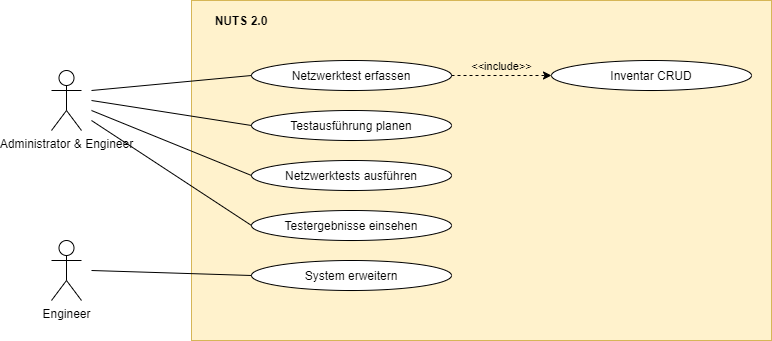
\includegraphics[scale=0.5]{\vorlagenOrdner/Bilder/UseCaseDiagram}

\section{Nichtfunktionale Anforderungen}
	In diesem Kapitel werden die nichtfunktionalen Anforderungen an das Projekt behandelt.
	Es werden Aspekte und Anforderungen aus den Bereichen Änderbarkeit, Benutzbarkeit, Effizienz, Zuverlässigkeit, Betreibbarkeit und Sicherheit betrachtet.
	Die jeweiligen Aspekte werden in ihren Unterkapiteln genauer beschrieben.
	Es werden mögliche Szenarien beschrieben, die in der Erstellung oder dem Betrieb der Software auftreten können und bei der Architektur in betracht gezogen werden.

	\subsection{Änderbarkeit}
		Aufwand, der zur Durchführung von vorgegebenen Änderungsarbeiten benötigt wird.
		Unter Änderungen gehen Korrekturen, Anpassungen oder Veränderungen der Umgebung, Anforderungen oder funktionalen Spezifikation.
		Gemäss ISO 9126 gehören zur Änderbarkeit folgende Teilmerkmale:
		
		\subsubsection{Analysierbarkeit}
			Aufwand, der benötigt wird, um das System zu verstehen, z.B. um Ursachen von Versagen oder Mängel zu diagnostizieren oder Änderungen zu planen.

		\subsubsection{Modifizierbarkeit}
			Wie leicht lässt sich das System anpassen, um Verbesserungen oder Fehlerbeseitigungen durchzuführen.

		\subsubsection{Stabilität}
			Wahrscheinlichkeit, dass mit Änderungen unerwartete Nebenwirkungen auftreten.

		\subsubsection{Testbarkeit}
			Wie gross wird der Aufwand, bei Änderungen die Software zu prüfen.

		\subsubsection{Szenario: Neue Netzwerkschnittstelle}
			Wenn zum bestehenden System eine neue Netzwerkschnittstelle definiert werden soll, so muss die dafür notwendige Software innerhalb von einer Arbeitswoche entwickelt, integriert und in Betrieg genommen werden können.

			\begin{tabularx}{\textwidth}{lX}
				\toprule
				Qualitätsziele & Flexibilität, Erweiterbarkeit, Anpassbarkeit, Austauschbarkeit  \\
				\midrule
				Geschäftsziel(e) & Software kann mit geringem Aufwand an geänderte Anforderungen angepasst werden  \\
				\midrule
				Auslöser & Es besteht eine andere Möglichkeit, auf ein Netzwerkgerät über eine Schnittstelle zuzugreifen, die nicht im System integriert und der implementierten Methode zu bevorzugen ist.  \\
				\midrule
				Reaktion & Die Software lässt sich von einem Entwickler in weniger als einer Woche um benötigte Komponenten erweitern.  \\
				\midrule
				Zielwert & 	Erweiterungen der Netzwerkschnittstellen sind innerhalb von 40 Personenstunden umsetzbar.  \\
				\bottomrule
			\end{tabularx}

		\subsubsection{Szenario: Verständlichkeit von generiertem Code}
			Generierter Code für die Netzwerktests ist leicht verständlich und manuell anpassbar.

			\begin{tabularx}{\textwidth}{lX}
				\toprule
				Qualitätsziele & Verständlichkeit, Testbarkeit, Modifizierbarkeit  \\
				\midrule
				Geschäftsziel(e) &  Tester können den generierten Code für die Testsuites und die Testfälle leicht verstehen und ihren eigenen Bedürfnissen anpassen. \\
				\midrule
				Auslöser & Ein Netzwerengineer möchte an der Software Änderungen vornehmen und dafür die Tests anpassen.  \\
				\midrule
				Reaktion & Die Testsuites und der Testcode für die Netzwerkeinstellungen werden durch einen Test-Generator in möglichst einfacher Form generiert. \\
				\midrule
				Zielwert & Tester und Entwickler können die generierten Tests in weniger als 30 Minuten verstehen und einfache Anpassungen vornehmen. \\
				\bottomrule
			\end{tabularx}

		\subsection{Scenario: Schnelle Fehlerlokalisierung}
			Die Ursache von fehlgeschlagenen Tests (Software-Unittests) lässt sich in kurzer Zeit lokalisieren.

			\begin{tabularx}{\textwidth}{lX}
				\toprule
				Qualitätsziele & Schnelle Fehlerbehebung, Änderbarkeit, Anpassbarkeit, geringes Risiko bei Erweiterungen  \\
				\midrule
				Geschäftsziel(e) & Entwickler können das Programm einfach anpassen und erkennen im Fehlerfall schnell, was nicht funktioniert hat.  \\
				\midrule
				Auslöser & Eine Änderung im Code führt zu Fehlnern in der Ausführung.  \\
				\midrule
				Reaktion & Wenn ein Fehler dazu führt, dass die Softwareausführung fehlschlägt, kann ein Entwickler aufgrund von Fehler- und/oder Log-Nachrichten die Ursache in kurzer Zeit lokalisieren.  \\
				\midrule
				Zielwert & Fehlerlokalisierung findet durchschnittlich in weniger als 10 Minuten statt.  \\
				\bottomrule
			\end{tabularx}

	\subsection{Benutzbarkeit}
		Zeitlicher Aufwand, der für die Erlernung der Benutzung des Programms benötigt wird. Die User werden hierfür in spezifische Nutzergruppen mit festgelegten Fähigkeiten unterteilt.
		
		\subsubsection{Verständlichkeit}
			Aufwand für den Nutzer, die Konzepte und Menüführung der Anwendung zu verstehen.

		\subsubsection{Erlernbarkeit}
			Aufwand für den User, sich ohne Vorwissen in das System einzuarbeiten.

		\subsubsection{Bedienbarkeit}
			Aufwand für den Benutzer, die Anwendung zu bedienen.

		\subsubsection{Szenario: Einfachheit der Testdefinitionen}
			Die Definitionen von Tests in YAML sind so aufgebaut, dass ein User in kurzer Zeit die Struktur und den Aufbau versteht und eigene Tests implementieren kann.
			
			\begin{tabularx}{\textwidth}{lX}
				\toprule
				Qualitätsziele & Produktivität, Einfachheit, Verständlichkeit \\
				\midrule
				Geschäftsziel(e) & Einarbeitung in die Testdefinition erfolg möglichst einfach und benötigt nur geringes Vorwissen.  \\
				\midrule
				Auslöser & Ein Nutzer, welcher keine Erfahrung im Umgang mit der Software hat, möchte eigene Tests definieren.  \\
				\midrule
				Reaktion & Benutzer können sich schnell in die Testdefinitionen einlesen und rasch eigene Tests definieren, vorausgesetzt, sie haben Kenntnisse des Netzwerkes.  \\
				\midrule
				Zielwert & Ungeschulte Nutzer verstehen innerhalb von durchschnittlich 30 Minuten die Struktur und den Aufbau der Testdefinitionen und sind in der Lage, eigene Tests zu erstellen.  \\
				\bottomrule
			\end{tabularx}
			
		\subsubsection{Szenario: Hinweis auf Fehleingaben}
		Fehlerhafte Eingaben werden vom System ignoriert und der Benutzer wird auf die falsche Eingabe hingewiesen. Das Programm führt fehlerfreie Programmteile unabhängig von den Fehlern durch.
			
		\begin{tabularx}{\textwidth}{lX}
			\toprule
			Qualitätsziele & Robustheit, Verständlichkeit, Fehlertoleranz.  \\
			\midrule
			Geschäftsziel(e) & Fehleingaben führen nicht dazu, dass die Tests nicht mehr durchgeführt werden können.  \\
			\midrule
			Auslöser & Ein Benutzer macht einen Fehler bei der Testdefinition und startet das Programm.  \\
			\midrule
			Reaktion & Das Programm führt alle korrekten Tests durch und informiert den Benutzer, dass es fehlerhafte Tests gibt, die nicht durchgeführt werden können. Die Hinweise werden im Report und auf der Konsolenausgabe geschrieben.   \\
			\midrule
			Zielwert & Tests sind einzeln gekapselt und werden unabhängig voneinander durchgeführt. Falscheingaben werden vom Programm detektiert und im Testreport sowie auf der Konsolenausgabe erwähnt.  \\
			\bottomrule
		\end{tabularx}
		
	\subsection{Effizienz}
	Mit Effizienz ist die 'performance efficiency' gemeint, d.h. das Verhältnis zwischen dem Leistungsniveau der Software und den eingesetzten Hardwarekomponenten. 
	Andere Beschreibungen umfassen: Skalierbarkeit, Speicherbedarf, Verarbeitungsgeschwindigkeit, Antwortzeit etc.
	Teilmerkmale nach ISO 9126:

		\subsubsection{Zeitverhalten}
		Dauer für Verarbeitung und Antwortzeit sowie Durchsatz bei der Ausführung des Programms

		\subsubsection{Verbrauchsverhalten}
		Wie viel Speicherbedarf hat das Programm, wie lange werden Betriebsmittel in Anspruch genommen und welche Hardwarekomponenten werden benötigt.

		\subsubsection{Szenario: Schnelle Erzeugung der Netztestdaten}
		Nach der Erstellung von Testdefinitionen können die Netztests ohne lange Wartezeiten erstellt werden um eine rasche Arbeitsweise zu garantieren.
			
		\begin{tabularx}{\textwidth}{lX}
				\toprule
				Qualitätsziele & Performanz, Laufzeitverhalten, Flexibilität, Geschwindigkeit  \\
				\midrule
				Geschäftsziel(e) & Die Zeit zwischen der Erstellung und der Durchführung von Tests wird gering gehalten.  \\
				\midrule
				Auslöser & Ein Benutzer erstellt Netztests und möchte diese rasch in das System einspeisen.  \\
				\midrule
				Reaktion & Tests werdem vom Testgenerator erstellt, so dass die Wartezeiten für Benutzer möglichst gering sind.  \\
				\midrule
				Zielwert & Netztests werden in weniger als 10 Sekunden generiert.  \\
				\bottomrule
			\end{tabularx}

		\subsubsection{Szenario: Optimierte Durchführung von Tests}
		Die Tests werden möglichst parallel abgearbeitet und nur dann seriell durchgeführt, wenn eine asynchrone Ausführung zu Störungen im Netzwerk führen würden. 
		
		\begin{tabularx}{\textwidth}{lX}
			\toprule
			Qualitätsziele & Effizienz, geringe Störung im zu testenden Netzwerk, Robustheit  \\
			\midrule
			Geschäftsziel(e) & Die Durchführung von Netzwerktests führt nicht zu Performanzeinbussen im Netzwerk.  \\
			\midrule
			Auslöser & Es werden mehrere parallelisierbare (z.B. Ping) und mehrere performanzstörende (z.B. Traffic-Test) Tests definiert.  \\
			\midrule
			Reaktion & Parallelisierbare Tests werden asynchron durchgeführt. Alle Tests, die das Netzwerk stören können werden nacheinander abgearbeitet. \\
			\midrule
			Zielwert & Es entstehen maximal 30\% Performanzeinbussen im Netzwerk während die Tests durchgeführt werden.  \\
			\bottomrule
		\end{tabularx}

	\subsection{Zuverlässigkeit}
	Unter Zuverlässigkeit versteht man die Fähigkeit der Software, unter festgelegten Bedingungen die Funktionalität über einen definierten Zeitraum zu gewährleisten
	
		\subsubsection{Reife}
		Geringe Ausfallhäufigkeit durch Fehlzustände.

		\subsubsection{Fehlertoleranz}
		Die Software ist in der Lage, trotz Fehlern ihr spezifiziertes Leistungsniveau beizubehalten.

		\subsubsection{Wiederherstellbarkeit}
		Im Fehlerfall können betroffene Daten wiederhergestellt und die Funktionalität wieder aufgenommen werden.

		\subsubsection{Szenario: Tests lassen sich auf der Netzwerkseite nicht ausführen}
		Falls ein Test auf dem jeweiligen Netzwerkgerät nicht erfolgreich durchgeführt werden kann, läuft das Programm weiter und definiert den dazugehörigen Netzwerktest als nicht bestanden.
		
		\begin{tabularx}{\textwidth}{lX}
			\toprule
			Qualitätsziele & Robustheit, Behandlung Infrastrukturbedingter Fehler.  \\
			\midrule
			Geschäftsziel(e) & Das System führt alle Tests unabhängig voneinander durch. Wenn ein Test zu einem Fehler führt, weil z.B. ein falsches Netzwerkgerät angegeben wurde, wird dieser Test unabhängig von allen anderen Tests fehlschlagen.  \\
			\midrule
			Auslöser & Test lässt sich auf spezifizierter Infrastruktur nicht ausführen.  \\
			\midrule
			Reaktion & Test schlägt fehl und mögliche Ursachen werden im Report und in der Konsole angezeigt. Alle anderen Tests laufen durch.  \\
			\midrule
			Zielwert & Das Fehlschlagen eines Tests fürht nicht zum Programmabbruch.  \\
			\bottomrule
		\end{tabularx}

	\subsection{Betreibbarkeit}
	Die Betriebbarkeit wird in der ISO 9126 nicht definiert. Die ISO spezifiziert aber mehrere Teilmerkmale, die unter dem Begriff Betreibbarkeit zusammengefasst werden können:

		\subsubsection{Analysierbarkeit}
		Aufwand, der benötigt wird, um den Code zu analysieren, um im falle eines Versagens dessen Ursachen zu diagnostizieren oder um Änderungen zu planen und durchzuführen.

		\subsubsection{Installierbarkeit}
		Aufwand, das Programm auf einem frisch aufgesetzten Gerät laufen zu lassen.

		\subsubsection{Übertragbarkeit}
		Kann die Software von einer Umgebung auf eine andere übertragen werden. 
		Als Umgebung zählen Hardwarekomponenten, Softwarekomponenten, Organisatorische Umgebungen oder Betriebssysteme. 

		\subsubsection{Austauschbarkeit}
		Aufwand und Möglichkeit, die Software anstelle einer anderen in deren spezifizierten Umgebung laufen zu lassen.

		\subsubsection{Koexistenz}
		Fähigkeit der Software, neben anderen Programmen mit ähnlichen oder übereinstimmenden Funktionen zu arbeiten.

		\subsubsection{Szenario: Einfache Installation auf einem neuen Gerät}
		Das Programm lässt sich auf einem neuen Gerät ohne grossen Mehraufwand installieren, ohne dass die Funktionalität des Geräts beeinflusst wird.

		\begin{tabularx}{\textwidth}{lX}
			\toprule
			Qualitätsziele & Einfachheit, Portierbarkeit, Benutzbarkeit  \\
			\midrule
			Geschäftsziel(e) & Die Installation der Software ist so einfach, dass sie innert kurzer Zeit und/oder automatisiert durchgeführt werden kann.  \\
			\midrule
			Auslöser & Die Testsoftware soll auf einem frisch aufgesetzten Gerät installiert werden.  \\
			\midrule
			Reaktion & Installationszeiten sind gering, benötigen wenige bis keine weiteren Softwarekomponenten oder lässt sich mit einigen Kommandozeilenbefehlen automatisch installieren.  \\
			\midrule
			Zielwert & Die Software wird mit einer Installationsanleitung ausgeliefert, die einfach und verständlich die Inbetriebnahme des Programms erklärt. Abhängigkeiten zu anderen Softwarekomponenten werden bewusst gering gehalten um eine einfache Installation mit weniger als 30 Minuten Zeitaufwand zu gewährleisten.  \\
			\bottomrule
		\end{tabularx}


	\subsection{Sicherheit}
	In dieser Sektion werden Sicherheitsanforderungen beschrieben. 
	Verschlüsselung, Privacy und der Umgang mit Passwörtern.

		\subsubsection{Verschlüsselung von Datenübertragungen}
		Die Netzwerktest werden über eine Verschlüsselte Verbindung durchgeführt, die dem aktuellen Stand der Technik entspricht.

		\subsubsection{Umgang mit Passwörtern}
		\textcolor{red}{Zum Zeitpunkt der Erstellung dieses Dokuments ist noch nicht klar, wie mit Passwörtern sicher umgegangen werden soll. Die Usability setzt voraus, dass der Testdurchführer nicht für jeden Test einzeln ein Passwort eingeben muss, Security-verhaltensweisen verbieten aber das Abspeichern von Passwörtern als lesbaren Text.}

\end{document}